% vim:set et sw=2 ts=4 tw=72:
% Jun 24, 2017


The results show conclusive results; the DAG visualization is unable to
adequately provide users with an explanation of the changes being made
in the repository, the DAG visualizatoin is not easily understood, and
is unable to provide summarizations of the changes being made at a
merge. Meanwhile, the \mt visualization is better able to provide an
explanation of how a commit is integrated, along with better
summarization. In this section, we discuss some observations, threats to
the validity, and comments made by the participants during the study
followed by discussion about modifications to the original algorithm to
help generalize it for more repositories, concluded with future work.

% TODO: Future work?

\subsection{Observations}
\label{sub:observations}

% \dmg{I think you mean challenge using gitk, right? so be explicit}

During the course of the study, we noticed an issue that was consistent
among the participants when using Gitk; the most difficult challenge was
identifying the master branch of the repository. Many participants would
identify the tag as being the ``master branch'', but a tag is not a
branch. The visualization of the DAG does not provide any notion of
which branch being shown is the master branch. The default assumption is
that the first branch on the left is the master branch, but this is not
a good assumption. Furthermore, the visualization in Gitk is not
consistent, the ordering of the branches changes between runs, so
identifying the branch once will not guarantee that it will be
identifiable after restarting Gitk.

If users were able to easily identify the master branch using the
visualizations of the DAG, the results of the study would likely be very
different. This would certainly be the case for the single-commit tree;
it is trivial to summarize information about a single item, but
identifying that there was only a single commit in the tree was
non-trivial. This information is important because many trees contain a
single commit, and the structure of these trees is identical to the
structure of flat trees. Flat trees are the most common branching
structure in the repository, with the root being the parent to all of
the other nodes in the tree; to improve summarization and comprehension
of these trees, it would likely by sufficient to indicate the master
branch in the DAG visualization.

While, in general, the participants of the study preferred using \tool
to Gitk, there were some noticeable usability issues in \tool. The most
prominent issue being the navigation within the tree visualizations. The
participants expected that the tabs would update when they clicked on a
node in the tree, instead of having to click the link to the commit
after clicking the node. This was true in both the \rt tree and the Pack
tree. The second major usability issue was the inconsistency between the
list tree and the other tree visualizations. The list tree is rooted at
the repository event that the user is current looking at, while the
other tree visualizations show the entire tree, and use bright orange to
highlight the current node.


\subsection{Comments From a Release Manager}
\label{sub:comments_from_a_release_manager}

One participant in the study worked as a release manager for more than
three years, working with both SVN and CVS repositories, but had little
experience with git. This subsection contains improvements made by this
participant during the study and afterward.

Contributors making merges need to understand more than just what merges
a commit was collected into before reaching the repository of the
contributor. It is also important to understand order that the related
commits were made, as the order tells the story of what the developer
was thinking as they were writing the changes. The current \mt model
does not order the commits, simply placing them randomly. This is the
primary reason behind this participant's request to use both
simultaneously. \tool is able to help with the aggregation of the
information, and provide a better understanding of the next merge
involved in integrating this commit, but the DAG visualization in Gitk
provides the full story of the commit instead of hiding it behind a
layer of abstraction.

The comments from this participant were very insightful, and will assist
in improving the model in the future.

\subsection{Threats to Validity}
\label{sub:threats}

\textbf{Internal Threats:}

The repository contains many commits, of which we only chose two. The
commits chosen were randomly selected to be representative of those in
the repository. Additional commits could be added, but this would
include additional time costs during the study.

The answers provided by the participants to earlier tasks were not
taken into account for determining the accuracy. If the participant was
unable to determine the correct commits for the tree within the
conceptual task group, the summarization results would be recorded as
wrong, even if the summarization they provided was correct for the set
of commits selected to be part of the tree. A further study could be
done where the correct answer was provided to the participant after each
task so that errors would not propagate between tasks.

To mitigate the effects of order-bias, the order the tasks were
performed, the tools were used, the commits were studied was shuffled
between participants. A single participant is affected by the effect,
but this should be mitigated by the results from other participants.

We were only able to work with 12 participants. We apply various
statistical tests to ensure that our findings are reasonable.

\textbf{External Threats:}

While git includes Gitk and git log provides a visualization of the DAG
with \verb|git log --graph|, many of the participants in our study were
unfamiliar with the DAG visualizations shown by these tools. Other tools
may provide better summarizations and visualizations, but we are unaware
of any. We investigated the gui tools for Linux on the git
website\footnote{\url{https://git-scm.com/download/gui/linux}}, but none
of the tools, with the exception of Gitk and git log, were able to
produce a visualization of the DAG for the Linux repository.
Investigating the tools more deeply, it appears that GitKraken is the
most popularly cited git client. The visualization provided by GitKraken
was centered around the same DAG metaphor used by git log. GitKraken was
unable to produce a visualization for the Linux repository on our
system. Inspecting these tools on smaller repositories show that the
visualizations of the DAG were very similar to the visualization in
Gitk.

% A possible
% reason for this may be that unless a repository reaches a sufficient
% complexity, both in branching and number of commits, these tools are
% unnecessary for the normal operation of git. Furthermore, fear of the
% complexity caused by branching may cause personal and academic
% repositories to have relatively simple structures. While they were
% unfamiliar with the DAG structure, these users were also unfamiliar with
% the \mt model, and were still able to better understand and summarize
% the repository using \tool.

\subsection{Generalization}
\label{sub:generalization}

Seeing that the visualizations of the \mt model are able to assist users
with understanding how commits are integrated, we continue by looking at
ways of improving the algorithm for faster operations, and making the
conversion from DAG to \mt feasible over the internet.

The problem of identifying the master branch is the most difficult, and is
not possible without heuristic approaches. The master branch can be
confounded by \foxtrot merges, which change the order of the
parents in the parent list of a merge. Other than the ordering of the
parent list, git has no other way to determine which commits are on the
master branch of the repository. For the purpose of this discussion, we
will assume that we can rely on the order of the parent list to be
correct, and that \foxtrot{s} do not occur. Furthermore, merge
information is lost in the event of fast-forward merges, which collapse
the branch into the current branch.

\begin{algorithm}
  \caption{Computing the generalized Merge Tree}
  \label{alg:generalized}
  \begin{algorithmic}[1]
    \Function{Phase 1}{initial commit $root$} : updated tree
    \State $openBranches \gets 0$
    \State $Q \gets root$
    \Do
    \State $cur \gets Q.dequeue$
    \State $parents \gets cur.parents$
    \State $openBranches \gets openBranches + parents.length - 1$
    \For{$index, parent \in parents$}
    \If{$parent.depth$ is $undefined$}
    \State $parent.depth \gets cur.depth + index$
    \ElsIf {$cur.depth > parent.depth$}
    \State $openBranches \gets openBranches - 1$
    \ElsIf {$cur.depth < parent.depth$}
    \State $openBranches \gets openBranches - 1$
    \State $parent.depth \gets cur.depth$
    \EndIf
    \State $parent.children \gets cur$
    \If{$parent$ has not been visited}
    \State $Q \gets parent$
    \State $parent.visited \gets True$
    \EndIf
    \EndFor
    \doWhile{$Q$ not empty and $openBranches \ne 0$ }
    \EndFunction

    \Function{Phase 2}{initial commit $root$} : Merge tree
    \State $tree.root \gets root$
    \State $Q$ // Empty Queue

    \State $parents \gets root.parents$
    \State $parents \gets tail\ parents$
    \For {$parent \in parents$}
    \State $realParent \gets min(\forall child \in parent.children,\ parent.depth >= child.depth)$
    \If {$realParent$ is $root$}
    \State $root.children \gets parent$
    \State $parent.parent \gets root$
    \State $Q \gets parent$
    \EndIf
    \EndFor

    \While{$Q$ not empty}
    \State $cur \gets Q.dequeue$
    \State $parents \gets cur.parents$
    \For{$parent \in parents$}
    \State $realParent \gets min(\forall child \in parent.children,\ parent.depth >= child.depth)$
    \If {$realParent$ is $cur$}
    \State $cur.children \gets parent$
    \State $parent.parent \gets cur$
    \State $Q \gets parent$
    \EndIf

    \EndFor
    \EndWhile

    \EndFunction
  \end{algorithmic}
\end{algorithm}

The primary difference between the original algorithm and the
generalization is the main data structure. Algorithm~\ref{fig:alg}
is centered around the use of the stack, making it akin to a depth-first
traversal of the DAG with dynamic programming. The generalization in
Algorithm~\ref{alg:generalized} is based on the queue, making it akin to
the breadth-first traversal of the DAG.\@ While the final results of the
two traversals should not be different, the runtime properties are
different.

We will begin with a simplified description of the original algorithm.
The algorithm starts at the reference to the master branch. We will use
the term master branch loosely here, meaning any branch that has been
labeled in some way as being the main branch, this branch may have a
different name, but standard naming conventions call it the master
branch. Starting from the master branch label, we traverse the entire
master branch to the initial commit, recording the commit hash of every
repository event encountered.

The second phase iterates over every repository event, computing the
shortest distance to the master branch. For this reason, the entire
repository must be available to the algorithm. This is a dynamic
programming solution, centered around the call stack. The next node on
the shortest path to the master branch will become the parent of this
node in the tree.

If this algorithm is to be generalized into a dynamic, web-based, tool,
it may not be feasible to download every every repository event in the
repository in a reasonable period of time. We instead look toward a
breadth-first approach at limiting the number of repository events that
must be downloaded.

Focusing on the generalized algorithm (Algorithm~\ref{alg:generalized}),
the algorithm is broken into two phases. The first phase is where the
improvements take place. The first phase has three main goals; the first
is to track the master branch; the second goal labels the depth of each
repository event that is traverses, or how many merges the event is from
being merged; the third goal is to record the children of each
repository event. The first phase also begins the process of reversing
the DAG, by providing the candidate events that could possibly be the
real parent to this node. The first phase can terminate early, if it
reaches a point where all branches that it is following terminate. The
$openBranches$ metric on line 7 indicates how many branches are
currently being traversed. In line 11 through 15, we decrement the
$openBranches$, as this is the point where a branch occurs. The second
branch closing clause is necessary to handle the case when the depth was
incorrectly assigned, which can occur if there are more events on the
current branch than on the side branch.

\begin{table}[htpb]
  \centering
  \caption{Example traversal of the example DAG in
    Figure~\ref{fig:repoDAG} starting at merge 11.}
  \label{tab:ex_traversal}
  \begin{tabular}{cccc|cc}
    \toprule
    Current & Parents & Open Branches & Q       & Visited & Children\\\midrule
    -       & -       & 0             & 11      & 11:0    & \\
    11      & 4,9     & 1             & 4,9     & 4:0     & 11, 5\\
    4       & 1       & 1             & 9,1     & 9:1     & 11\\
    9       & 7,6,8   & 3             & 1,7,6,8 & 7:1     & 9, 8\\
    1       &         & 3             & 7,6,8   & 6:2     & 9\\
    7       & 5       & 3             & 6,8,5   & 8:3     & 9\\
    6       & 5       & 2             & 8,5     & 5:1     & 7, 6\\
    8       & 7       & 1             & 5       & 2:1     & 5, 3\\
    5       & 4,2,3   & 2             & 2,3     & 3:2     & 5\\
    2       & 1       & 1             & 3       &         & \\
    3       & 2       & 0             &         &         & \\
    \bottomrule
  \end{tabular}
\end{table}

In Table~\ref{tab:ex_traversal}, we follow the algorithm starting at
merge 11 from the example in Figure~\ref{fig:repoDAG}, recording the
current node, the parents of the current node, the open branches, and
the queue structure after updating. The visited column is not dependant
on the current step, but keeps track of the nodes that have been
visited, the depth, and the children of the corresponding node. When we
reverse the DAG, the children in this table will become the candidates
for being the parent of the corresponding node. For example, the parent
of node 7 may be resolved to either node 9 or node 8. In this case, the
shortest path to the master branch is through node 9.

The terminology surrounding the parent/child relationship gets very
confusing at the change between phase one and two because this is where
the roles switch. In phase 1, we are working with the DAG; in phase 2,
we are working with a structure that is neither a tree nor a DAG, but
can only be described as a directed graph.

The goal of the second phase is to resolve the tree from the directed
graph. We will refer to parents in the same sense as we would refer to
them in the tree form of the repository for the remainder of this
section. We have gathered the depths and possible parents (line 17), but
we need to remove the extra parents. Extra parents are culled in line 42
of the algorithm. Of the possible parents, we take the parent that is
closest to the root, but not beyond. This forces the real parent to
either be deeper in the tree, or on the same branch as the current node.
Line 30 to 37 are for bootstrapping the queue, ensuring that we are not
starting on an empty queue and is nearly identical to lines 41 to 48.

The construction of the tree becomes trivial now that we are able to
determine the parents and children for each node. Lines 44 and 45
perform this construction, adding the DAG parent to the tree children of the
current node, and the DAG parent's parent becomes the current node,
which was the DAG parent's child. We continue following the path until
we hit the root node, merging the commit into the master branch.

This algorithm relies heavily on the order of parents in the parent
list, but is able to trim the number of nodes that must be downloaded.
Furthermore, the resulting tree is able to show the order of commits,
telling the story of how a developer was working, before the set of
commits was merged. We developed a small Bitbucket plugin to test the
design and determine whether it was capable of producing \mt{s},
shown in Figure~\ref{fig:b_plugin}.

\begin{figure}[htpb]
  \centering
  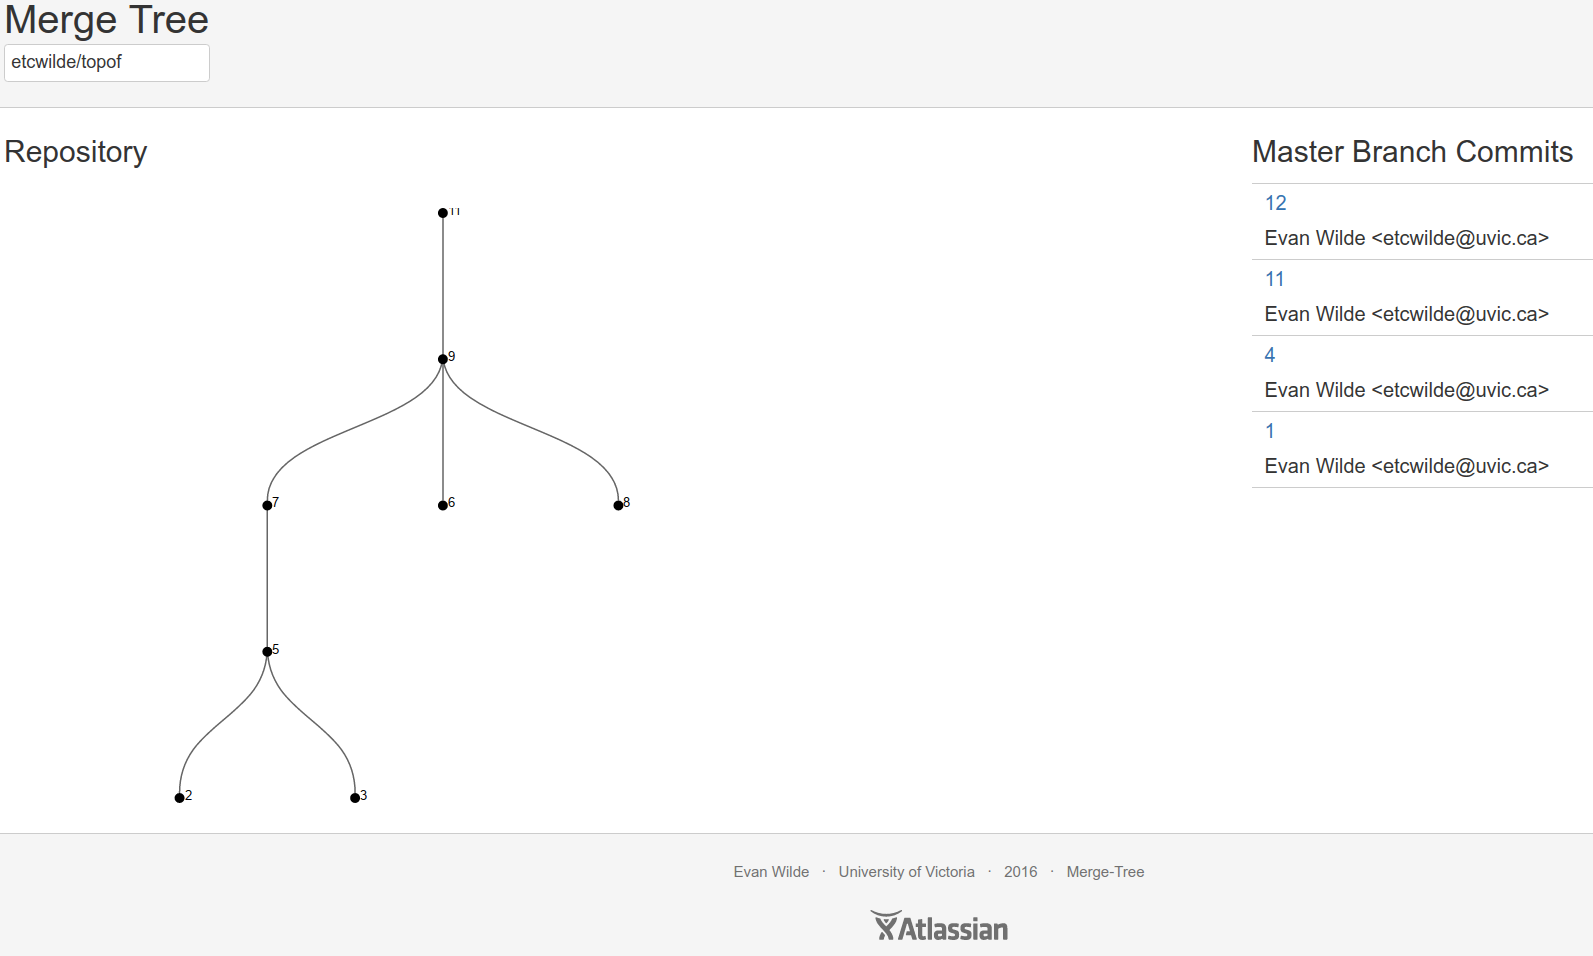
\includegraphics[width=\linewidth]{figures/plugin.png}
  \caption{Screen shot of the Bitbucket plugin showing the online tree
    computation of the repository shown in~\ref{fig:repoDAG}.}
  \label{fig:b_plugin}
\end{figure}


%%% Local Variables:
%%% mode: latex
%%% TeX-master: "userstudy"
%%% End:
